%\vspace{-0.1in}

\section{Adabot}
\label{sec:adabot}

%\vspace{-0.1in}

% In this section, we describe the prototype Adabot hardware, including the transformable wheel mechanism, along with the simulation environment utilized during evolutionary optimization.

% Hardware
% \subsection{Hardware}
% \paragraph{Hardware}
% \vspace{0.1in}
\noindent
\textbf{Hardware:}
%
The Adabot, pictured in \figref{fig:adabot}, is a prototype device that includes a Raspberry Pi 3 Model B (RPi) as its main control board.
%
The RPi was chosen for its ability to run the Robot Operating System (ROS)~\citep{Quigley.ICRAOSS.ROS.2009}, which Adabot uses to deploy its software systems.
%
The size of an RPi constrains the minimum dimensions of the Adabot's chassis. Specifically, the chassis must be at minimum 8~\si{cm} by 8~\si{cm}.
%
\tblref{tbl:params-physical} lists all configurable parameters for Adabot's physical characteristics, where
$\mathit{WheelBase}$ and $\mathit{TrackWidth}$ denote the distance between the front and rear axles and the lateral distance between wheels, respectively, and $\mathit{StrutCount}$ parameter indicates the number of struts per wheel.

%\vspace{-0.22in}

\begin{table}[hb]
    \centering
    \caption{Adabot Physical Parameters}
    \label{tbl:params-physical}
    \begin{tabular}{@{}ll@{}}
        \toprule
        \textbf{Name} & \textbf{Range}\\
        \midrule
        $\mathit{WheelBase}$    & \numrange{8}{16}~\si{cm}\\
        $\mathit{TrackWidth}$    & \numrange{8}{16}~\si{cm}\\
        $\mathit{WheelRadius}$ & \numrange{2}{3}~\si{cm}\\
        $\mathit{StrutCount}$        & \numrange{0}{7}\\
        \bottomrule
    \end{tabular}
\end{table}

% \vspace{-0.1in}

Each of the four wheels is driven by its own DC gear-motor with magnetic encoders.
%
Likewise, each wheel includes a set of struts that can be extended and retracted by a linear servo.
%
For sensing, Adabot includes three forward facing distance sensors and an IMU (3-axis gyroscope, 3-axis accelerometer, and 3-axis magnetometer).
%
Finally, it uses a 2.4 GHz wireless communication module and is powered by a 2200 mAh battery pack, which provides roughly two hours of operating time.


% Extension
% \subsection{Extender Mechanism}
% \paragraph{Extender Mechanism}
% \vspace{0.1in}
\noindent
\textbf{Strut Extension:}
%
\figref{fig:wheel-extender} depicts the strut extension process.
%
This mechanism enables the wheel to exhibit a range of characteristics.
%
With the struts fully retracted, the wheels operate conventionally; when extended a small amount, the struts act as tire studs; and with the struts fully extended, each wheel resembles a legged-wheel.
%
% \red{The radius of the wheel and the number of struts are both free parameters that can be evolved during optimization.}
%
% For this study, the most important aspect of this mechanism is that
Due to limitations of the design, the maximum extension of the struts is equal to the wheel's radius minus 1~\si{cm} ($\mathit{MAXEXT} = \mathit{WheelRadius} - 1~\si{cm}$).
%
For a more detailed discussion of Adabot's software and wheel extension mechanism, and an example of evolving Adabot with ROS and Gazebo (a simulation environment tightly coupled with ROS)
% ~\citep{Koenig.IROS.Gazebo.2004}
see our preliminary study~\citep{Clark.2017.SSCI.Adabot}.



\begin{figure}[!ht]
    \centering

    % \vspace{-0.08in}

    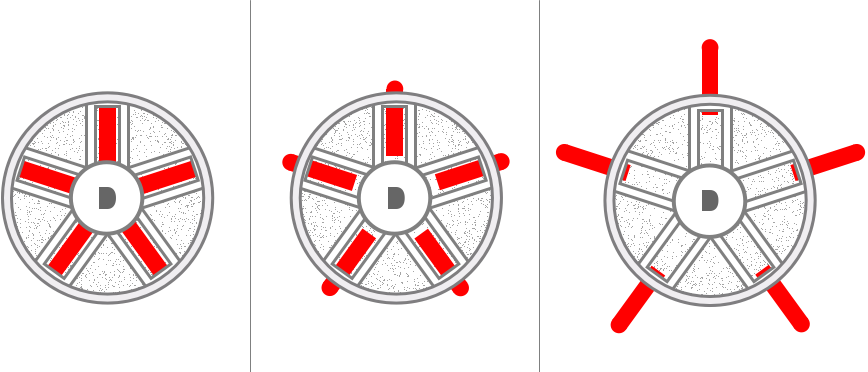
\includegraphics[width=0.8\columnwidth]{figures/3-adabot/extension-mechanism.png}

    % \vspace{-0.15in}

    \caption{Illustration of Adabot's wheel extension mechanism, where the struts are fully retracted (left), partially extended (middle), and fully extended (right).}
    \label{fig:wheel-extender}

    % \vspace{-0.18in}

\end{figure}

% Simulation
% \subsection{Simulation}
% \paragraph{Simulation}
% \vspace{0.1in}
\noindent
\textbf{Simulation:}
%
% As is the case for most ER studies, we use simulation during the optimization process.
%
An image of the simulation environment is shown in \figref{fig:simulation-environment}.
%
% To populate the environment with obstacles, we generate 40 boxes with random dimensions, positions, and densities.
The environment is populated by generating 40 boxes with random dimensions, positions, and densities.
%
If a newly generated box collides with an existing box it is removed from the simulation. We see on average 31 boxes placed in the environment.
%
Box heights range from \numrange{2}{5}~\si{cm}, which is high enough (compared to $\mathit{WheelRadius}$ values) to drastically reduce mobility for a wheeled robot~\citep{Quinn.IROS.Whegs.2002}.
%
Moreover, rather than each box being in a fixed position, it is possible for the Adabot to push a box (depending on its size and density).


For this study, we are using the Dynamic Animation and Robotics Toolkit (DART)\footnote{\url{https://dartsim.github.io/index.html}}.
%
DART is specifically designed for robotics applications,
% (unlike the Open Dynamics Engine\footnote{\url{https://bitbucket.org/odedevs/ode}}, which we've used in the past)
and is comparable in speed (if not faster) than common alternatives~\citep{Mouret.2017.SimER.Simulation}.
%
% In this study, we do not simulate noise, and we assume that the robot has direct access to its global position and rotation. Essentially, we are mimicking a lab setup with an overhead camera that communicates directly with the robot.
%
% In previous work, we used the ROS/Gazebo system for simulation, however, ROS was unnecessary for this study as we were not relying on any of its packages (e.g., \emph{robot_localization}~\cite{Moore.IAS.Robot-localization.2014}).


\begin{figure}[!ht]
    \centering

    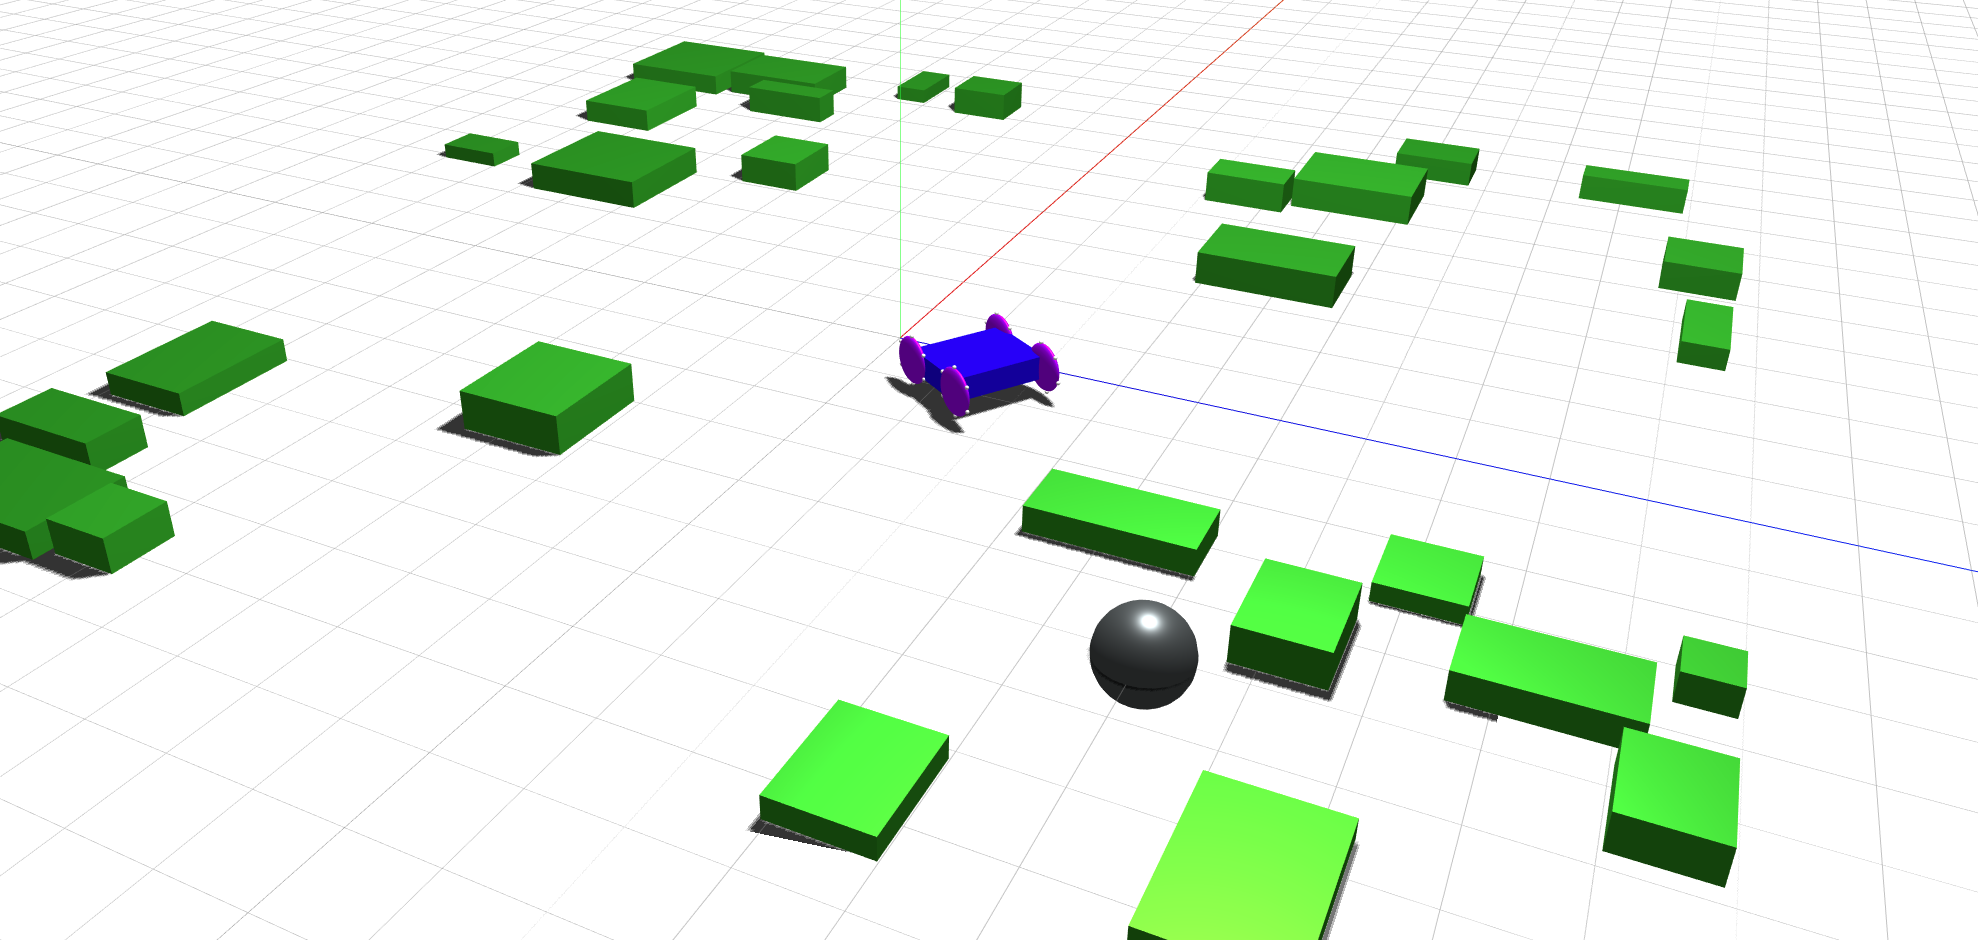
\includegraphics[width=0.8\columnwidth]{figures/3-adabot/environment.png}
    % \fbox{\crule[white]{\columnwidth}{2cm}}

    % \vspace{-0.12in}

    \caption{An example environment including randomly generated obstacles. The current way-point is shown as a dark gray sphere, and the robot starts at the origin facing in the positive x-axis (away from the way-point, along the red axis line).}
    \label{fig:simulation-environment}

    % \vspace{-0.15in}

\end{figure}

% Control Properties
% \subsection{Way-Point Navigation Control}
% \paragraph{Way-Point Navigation Control}
% \vspace{0.1in}
\noindent
\textbf{Way-Point Navigation Control:}
%
Adabot is a skid-steer style robot--it turns by rotating its left and right wheels at different rates. Although each wheel and wheel strut set can be controlled independently, in this study we only have three control outputs: (1) an angular rate for the left wheels, (2) an angular rate for the right wheels, and (3) a single extension amount for all four sets of struts.
%
For Adabot to aid during a search and rescue operation, it must be able to successfully \emph{cover} (completely search) its designated area.
%
A simplified version of this task, called \emph{way-point navigation}, is considered during evolutionary optimization.
%
For this task, a UGV must visit a set of way-points in sequence.
%
% Way-point navigation is the task that we consider during evolutionary optimization.
% We consider way-point navigation


% \vspace{0.1in}
\noindent
\textbf{FSM Control:}
The hand-designed FSMs for this task are depicted in \figref{fig:fsm}.
%
This FSM includes two independent actions: (a) directing the robot towards the next way-point by controlling the left and right wheels, and (b) extending the struts when the robot is experiencing reduced mobility due to an obstacle.
%
% The first action is handled by the three states shown in the top-half of the figure.
Essentially, the robot remains in the \emph{Forward} state as long as the angle between the heading of the UGV and the direction to the target ($\alpha_{\mathit{target}}$) is within some threshold.
%
Once the threshold is surpassed, the FSM transitions to either the \emph{Left} or \emph{Right} state.
%
In the \emph{Left} and \emph{Right} states, the robot will rotate in place until $\alpha_{\mathit{target}}$ is greater than $L.ToForwardThresh$ or less than $R.ToForwardThresh$, respectively, after which point the FSM transitions back to \emph{Forward}.
%
Threshold angles are shown in \figref{fig:fsm}(c).

\begin{figure*}[!ht]
    \centering

    % \includegraphics[width=0.6\columnwidth]{figures/4-simulation/state-machine.png}
    % \subfloat[]{\fbox{\crule[white]{0.4\columnwidth}{2cm}}}
    \subfloat[Direction Control]{%
        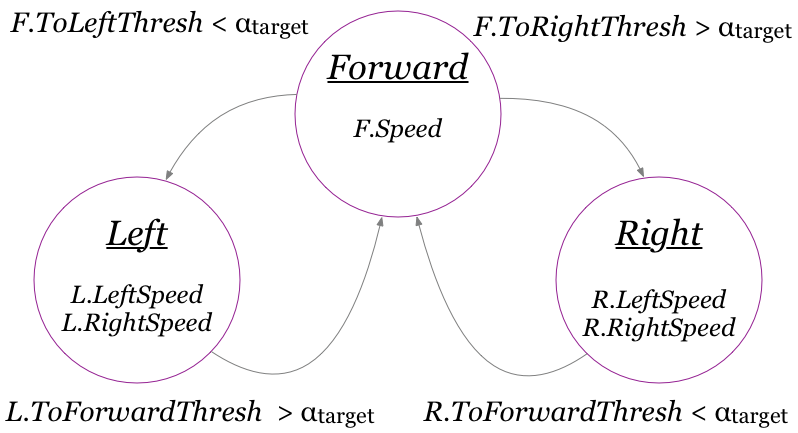
\includegraphics[width=0.45\textwidth,valign=c]{figures/3-adabot/FSM-direction.png}%
        % \vphantom{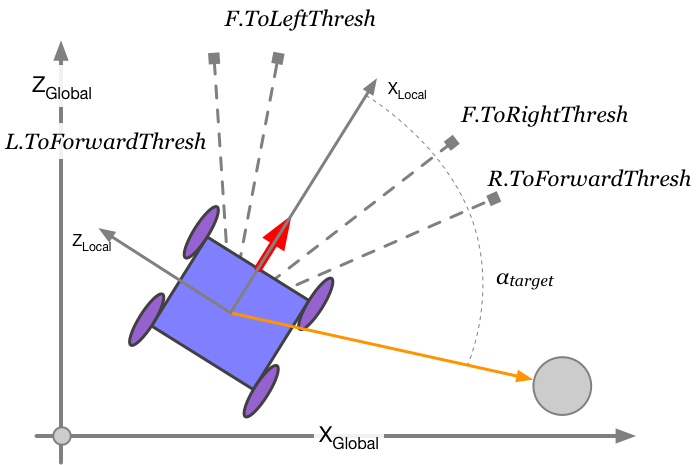
\includegraphics[width=0.3\textwidth,valign=c]{figures/3-adabot/scene.png}}%
    }
    \hfil
    \subfloat[Extension Control]{%
        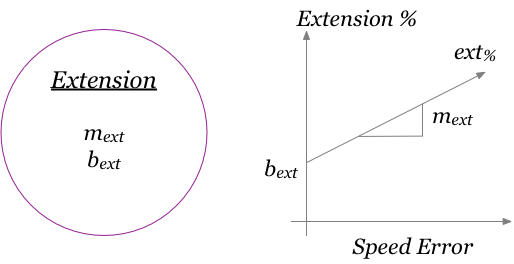
\includegraphics[width=0.45\textwidth,valign=c]{figures/3-adabot/FSM-strut.png}%
        % \vphantom{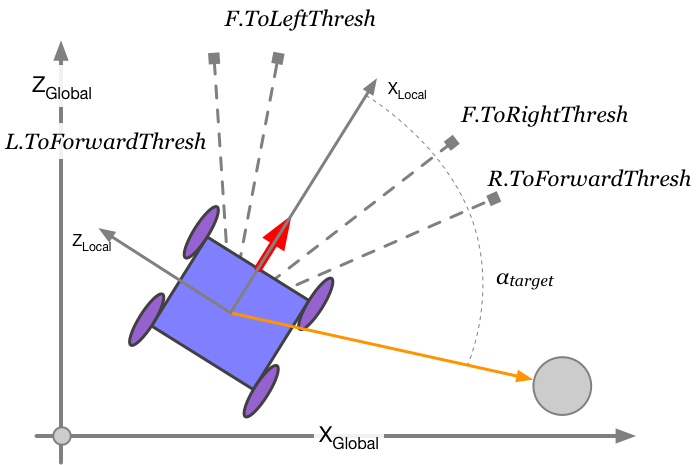
\includegraphics[width=0.3\textwidth,valign=c]{figures/3-adabot/scene.png}}%
    }

    % \hfil

    \subfloat[Environment Diagram]{%
        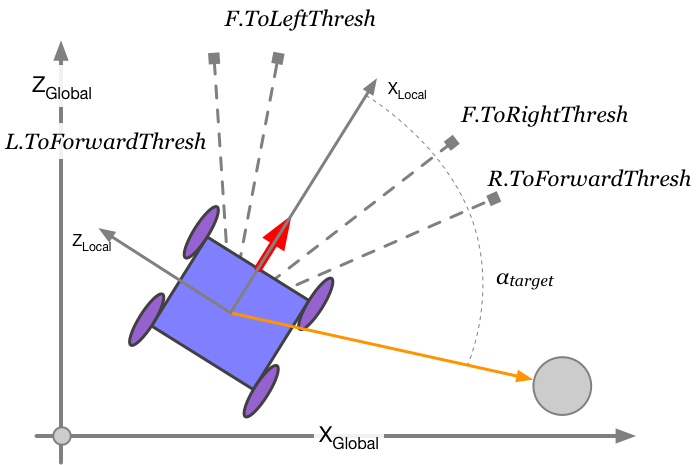
\includegraphics[width=0.65\textwidth,valign=c]{figures/3-adabot/scene.png}%
        % \vphantom{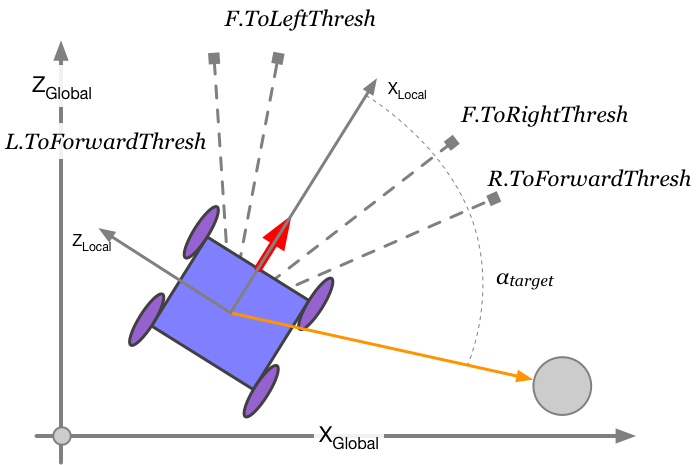
\includegraphics[width=0.3\textwidth,valign=c]{figures/3-adabot/scene.png}}%
    }

    % \vspace{-0.08in}

    \caption{(a) The FSM controlling the direction of the robot, (b) the single state controlling wheel struts, and (c) a diagram depicting the angles used to trigger transitions between states.}
    \label{fig:fsm}

    % \vspace{-0.15in}

\end{figure*}


To determine when, and by how much, wheel struts should be extended, we use a simple model based on the UGV's current error. Specifically, we calculate an expected linear ($v$) and angular ($\omega$) velocity (based on the wheel rates) using the following model:

% The second action, handling the wheel struts, is accounted for by the state shown in the lower part of \figref{fig:fsm}(a).
%
% This state calculates the expected linear and angular  speed using a simple differential drive model:

% \vspace{-0.12in}

\begin{align}
  v &= \frac{V_r + V_l}{2},\\
  \omega &= \frac{V_r - V_l}{\mathit{TrackWidth}}
\end{align}

\noindent
where $V_r$ and $V_l$ are the left and right wheel linear velocities,
% (depending on the left and right wheel rates, described below, as well as $\mathit{WheelRadius}$)
respectively, and $\mathit{TrackWidth}$ represents the distance between wheels on the same axle line (front or rear axles).
%
% As we are dealing with a noise-free, idealized simulation, this differential drive model has shown to be very accurate.
%
% It compares the expected speed to the actual speeds of the device, which are known exactly in simulation and can be measured accurately using an overhead camera setup in physical experiments, to calculate the scaled (between 0 and 1) absolute error values $v_e$ and $\omega_e$.
%
These calculated values (expected based on the differential drive model) are then subtracted from the actual linear and angular velocities values.
%
The difference value (the error between expected and actual velocities) are then scaled between 0 and 1 to produce $v_e$ and $\omega_e$, which are the scaled linear and angular velocities, respectively.
%
Error values are scaled between 0 and 1 and then filtered using exponential smoothing. Finally, they are used in the following equations to calculate the extension amount of all struts:

% \vspace{-0.2in}

\begin{align}
    \mathit{ext}_v &= m_{\mathit{ext}} \cdot v_e + b_{\mathit{ext}},\\
    \mathit{ext}_\omega &= m_{\mathit{ext}} \cdot \omega_e + b_{\mathit{ext}},\\
    \mathit{ext}_\% &= \max[\mathit{ext}_v, \mathit{ext}_\omega],\\
    \mathit{ext} &= \mathit{MAXEXT} \cdot \mathit{ext}_\%
\end{align}

\noindent
where $\mathit{ext}_v$ and $\mathit{ext}_\omega$ denote the extension amount calculated due to the linear and angular speed values, respectively. These two values are calculated using a linear equation with a configurable slope ($m_{\mathit{ext}}$) and intercept ($b_{\mathit{ext}}$).
%
The final extension amount ($\mathit{ext}$) is based on the maximum of these two values, and is calculated as a percentage of the maximum possible extension ($\mathit{MAXEXT}$).
%
In essence, the struts will be extended by an amount that is linearly proportional to the current error in speed (maximum between linear and angular error).
%
Thus, when Adabot encounters an obstacle that blocks it from moving according to the differential drive model, it will extend the struts in an effort to climb over any obstacles.


\begin{table}[thb]
    \centering
    \caption{Adabot FSM Parameters (Hand-Chosen)}
    \label{tbl:params-fsm}
    \begin{tabular}{@{}ll@{}}
        \toprule
        \textbf{Name} & \textbf{Range}\\
        \midrule
        $m_{\mathit{ext}}$ & (0.5) \numrange{0}{1}\\
        $b_{\mathit{ext}}$ & (0.5) \numrange{0}{1}\\
        $F.Speed$ & (20) \numrange{0}{20}~\si{\radian\per\second} \\
        $F.ToLeftThresh$ & (10) \numrange{0}{90}\si{\degree}\\
        $F.ToRightThresh$ & (-10) \numrange{-90}{0}\si{\degree}\\
        $L.LeftSpeed$ & (-20) \numrange{-20}{20}~\si{\radian\per\second} \\
        $L.RightSpeed$ & (20) \numrange{-20}{20}~\si{\radian\per\second} \\
        $L.ToForwardThresh$ & (5) \numrange{0}{90}\si{\degree}\\
        $R.LeftSpeed$ & (20) \numrange{-20}{20}~\si{\radian\per\second} \\
        $R.RightSpeed$ & (-20) \numrange{-20}{20}~\si{\radian\per\second} \\
        $R.ToForwardThresh$ & (-5) \numrange{-90}{0}\si{\degree}\\
        \bottomrule
    \end{tabular}
% \vspace{-0.2in}
\end{table}


%
\tblref{tbl:params-fsm} shows all configurable parameters for the FSM (hand-chosen values are shown in parentheses).
%
Aside from the first $m_{\mathit{ext}}$ and $b_{\mathit{ext}}$, each name in the table takes the following form: a capital letter representing a state in \figref{fig:fsm}(a) (\textbf{F}\emph{orward}, \textbf{L}\emph{eft}, or \textbf{R}\emph{ight}), followed by a period, followed by either an angular wheel rate or a angle threshold value also described in \figref{fig:fsm}(a).
%
Finally, to reduce vibration and potential damage to the wheel struts, the maximum angular rate of the wheels is linearly scaled down from 20~\si{\radian\per\second} to 4~\si{\radian\per\second} when the struts are fully extended.

% Table 2 originally here


% For this study we decided to use this single, simple state (based on just two configurable values) to reduce the number of factors that must be considered while comparing the FSM to the ANN.
%
% In future work we plan to extend this FSM to handle more complex tasks and exhibit more complex dynamics.
%
% One final, important note regarding Adabot's control system.
% To reduce vibration and potential damage to the wheel struts, the maximum angular rate of the wheels is linearly scaled down from 20~\si{\radian\per\second} to 4~\si{\radian\per\second} when the struts are fully extended.


% \vspace{0.1in}
\noindent
\textbf{ANN Control:}
As an alternative to the FSM controller, we evolve an ANN for the same task.
%
The neural network receives three inputs (each scaled between 0 and 1): (1) $\alpha_{\mathit{target}}$, (2) $v_e$, and (3) $\omega_e$.
%
Essentially, the ANN is given the same information as the FSM, and produces the same three output values (left and right wheel rates and an extension amount).
%
% For the sake of analyzing the evolved networks, we chose to make the ANN as simple as possible. Thus, the network is feed-forward and it does not include any hidden nodes.
%
In our preliminary work, we found hidden nodes were unnecessary for this task (the same strategies and fitness values were attained with and without hidden nodes).
%
The genome for our ANN includes 13 values: one integer value representing the activation function (logistic, hyperbolic tangent, or the rectified linear unit) and 12 values for the neural network weights (three inputs plus one bias for each of the three outputs).



% \subsection{Evolution}
% \paragraph{Evolution}
% \vspace{0.1in}
\noindent
\textbf{Evolution:}
%
For this study, we employ the Covariance Matrix Adaptation Evolution Strategy (CMA-ES)~\citep{Hansen.2003.EC.CMAES}.
%
In particular, we use pycma\footnote{\url{https://github.com/CMA-ES/pycma}} (developed by \citeauthor{Hansen.2003.EC.CMAES}), which
%
% CMA-ES
works well on real-valued problems and has support for handling integer values such as $\mathit{ExtCount}$.
%
% Although we experimented with several of the configurable parameters, we did not notice any positive results when varying values from their defaults.
